\documentclass[12pt,
bibtotoc,liststotoc,appendixprefix
twoside,paper=a4,headings=small]{scrbook}
%
% Packages
% -----------------------------------
\usepackage[
  paper=a4paper,
  left=12.5mm,
  right=25mm,
  top=25mm,
  bottom=50mm,
  bindingoffset=10mm]{geometry}		% Seitenr�nder und Bindungskorrektur einstellen
  
\usepackage{apacite} 				% Literatur-Referenzen: American Psycholog. Assoc.
\usepackage{natbib}					

\setcitestyle{round,aysep={}} 		% Indizierg. in runden Klammern, zw. Autor u. Jahr
%\usepackage[latin1]{inputenc} 		% Umlaute im Text
%\usepackage{ngerman}				% Rechtschreibg.
\usepackage[T1]{fontenc}
\usepackage{lmodern}				% Schriftfamilie
\usepackage{microtype}				% f�r die Mikrotypografie (besseres Schriftbild)
\usepackage[headsepline,footsepline]{scrpage2}

\usepackage{graphicx} 				% Grafiken einf�gen (pdf,png - aber jpg vermeiden)
\graphicspath{{./Bilder/}}          % Pfad zu den Bildern
\usepackage[export]{adjustbox}		%Positionieren von Bildern Tabellen
\usepackage{subfigure}				% L�sst Bilder nebeneinander darstellen
\usepackage{varwidth}
\usepackage{url}					% URL's formatieren (z.B. in Literatur) 
\usepackage[colorlinks,linkcolor=black,citecolor=black,urlcolor=black]{hyperref} 				% f�r Hyperlinks in PDF-Dokumenten
\usepackage{wrapfig}   
  
\usepackage{tabularx} 				% bessere Gestaltung von Tabellen
\usepackage{longtable} 		
\usepackage{multicol}				
\usepackage{multirow}
\usepackage{booktabs}
\usepackage{float}
\usepackage{framed}
\usepackage[labelfont=bf]{caption}

		
\usepackage[active]{srcltx}

\usepackage{listings}				% Algorithmen

\usepackage{mdwlist}				% Listen

\usepackage{setspace} 				% Zeileneinstellung
\newtheorem{mydef}{Merksatz}  		% Falls Beispiele, Merks�tze m. fortl. Nr. gebr. werden
\newtheorem{bsp}{Beispiel}

\usepackage{todonotes}				% zum Erstellen von ToDos im Editor

\usepackage{lscape}					% zum Rotieren von Seiten

\usepackage{amsmath}				% zum Schreiben von mathematischen Formeln

\usepackage{calc}


\usepackage{footnote}				% Fu�noten
\usepackage{tablefootnote}			% Fu�noten in Tabellen

%\clubpenalty = 10000
%\widowpenalty = 10000 \displaywidowpenalty = 10000

\hyphenation{voll-st\"andigen}		% Worttrennungen global definieren

\setcounter{tocdepth}{3}			% Ebenen, die im Inhaltsverzeichnis angezeigt werden

% Document
% -----------------------------------
\begin{document}
\parindent 0pt

\frontmatter 
    % Titelseite soll keine Kopf oder Fu�zeile haben
\thispagestyle{empty}

% Alle Elemente sollen zentriert sein


\begin{center}

\vspace*{-10mm}

%{\LARGE Freie Universit�t zu Berlin}\\

\vspace*{1cm}

\includegraphics[width=1.0\textwidth]{FULogo_Ausdruck_RGB}

\vspace*{1cm}

% Art der Arbeit => (Bachelorarbeit ,Diplomarbeit, Masterarbeit, Seminararbeit)
\Large \textbf{Masterthesis}\\ 

%\section*{\Large Masterthesis}

\vspace{1cm}

% Titel der Arbeit 
\LARGE \textbf{Inference of Boolean Networks considering real-life time 
course Data}\\ 

%\mdseries{Inference of Boolean Networks considering real-life time course Data}
%IBM Plex Serif Thin [OTF or TTF only] 

\vspace{1.5cm}

\Large Nina Valery Kersten\\


\parbox{120mm}{
\begin{large}
\begin{tabbing}
\textbf{Supervisors}\\\\
\hspace{.7cm} \= Prof. Dr. Heike Siebert\\
\hspace{.7cm} \= Prof. Dr. Alexander Bockmayr\\\\

\textbf{Advisor}\\\\
Phd. Robert Schwieger\\\\

\textbf{November 20, 2018} \\ 
\end{tabbing}
\end{large}
}

\end{center}
\clearpage{\pagestyle{empty}\cleardoublepage}
 			% Titelblatt
    \newpage
    \clearpage{\pagestyle{empty}\cleardoublepage}
    \thispagestyle{empty}


\vspace*{1cm}

\begin{center}
    \textbf{Abstract}
\end{center}

\vspace*{1cm}

\noindent 
%Give a short overview:
%Describe the Pipeline


    \newpage
    \clearpage{\pagestyle{empty}\cleardoublepage}
    \onehalfspacing                  	% Zeilenabstand ab hier 1.5 zeilig
    \tableofcontents 					% Inhaltsverzeichnis
    \clearpage{\pagestyle{empty}\cleardoublepage} 
    
    \listoffigures 					 	% Abbildungsverzeichnis
    \clearpage{\pagestyle{empty}\cleardoublepage}
    
    \listoftables						% Tabellenverzeichnis rein
    \clearpage{\pagestyle{empty}\cleardoublepage}
% -----------------------------------
\mainmatter 							% die einzelnen Kapitel
    \chapter{Introduction}

The development and functioning of a cell and an organism in general is a product of a complex cellular machinery. This machinery is compound by the interaction of genes, proteins, mRNA and many other substances to induce a cascade of extracellular signals transducted by mechanisms of the cell membrane,reaching the nucleus of the cell, initiating a transcription process that controls the production and abundance of proteins. Proper functioning of these networks is essential to the survival and adapation of all living organisms, while malfunctioning of these networks has been identified as the cause of various diseases \citep{An evaluation of methods for inferring boolean network from time-series data}.
To understand the behaviour of a biological system it is necessary to find and analyze the main important processes in a system in a dynamical manner. Therefore high-throughput techniques provide a big abundance of information about various biological interactions measured over a series of time. Biological information can be considered as different systems such as signal transduction, gene regulation, protein-protein-interaction or metabolism. These information are put in a network which can be yielded by several strategies like Baysian networks, Boolean regulatory networks, Ordinary differential equation models and Neural networks\citep{SAADATPOUR20133}.Once a network is constructed further anaylsis of the network by validating the network (e.g. pertubations like gene manipulation and external treatments, reductions etc.)can be done to figure out the main interactions whose disfunctions cause diseases.
This work is focused on the inference of a Boolean regulatory network, which is helpful to applicate tools like PyBoolNet and BoolFilter for further analysis of the inferenced network. This chapter describes the different kinds of biological data, what a Boolean Regulatory Network is as well as the algorithms to yield a network and how the performance of a algorithm can be measured.


\section{Biological Background}

Depending on the aim of a network inference the biological input data can be depicted by the interaction of proteins, genes and metabolic substances. In this section the intention of using different types of input data is explained and what potentially will be the occuring problems. Different types of biological input data provide different structures of the input data for further network inference algorithms. 
\newpage

\subsection*{Signal Transduction}

In the developement of multicellular organisms the action of extracellualr growth factors activate a cascade of intracellular signaling pathways. These pathways regulate major aspects of cell regulation like cell profileration, cell migration, cell differentiation,cell survival and cell death. To understand the developement of diseases (e.g. cancer) major prozesses (e.g. phosphorylation, ubiquitylation, methylation, etc.) of signal transduction pathways can be delightet by the prediction of a network . In signal transduction proteins are the nodes and directed edges represent interaction, where the biochemical modification of the regulatee is changed by the impact of the regulator. The concentration of signalling pathway underlies high fluctuation over time due to transcriptional and translational regulation, such that the inference of a network is a challenging task \citep{BIES:BIES20834}
%\citep{https://www.ncbi.nlm.nih.gov/pmc/articles/PMC3436851/}.


\begin{figure}[H]
\centering
%\setlength{\abovecaptionskip}{0pt}
\includegraphics[width=0.5\textwidth]{./Bilder/signaltransduction.pdf}
\setlength{\abovecaptionskip}{-10ex}
\caption[Signal Transduction]{\textbf{Signal Transduction.} An environmental signal (e.g. hormone) interacts with a cellular component, most often a cell-surface receptor. The information that the signal has arrived is then converted into other chemical forms, or transduced. The signal is often amplified before introducing a response. Feedback pathways regulate the entire signaling process.\citep{Berg JM, Tymoczko JL, Stryer L. Biochemistry. 5th edition. New York: W H Freeman; 2002. Chapter 15, Signal-Transduction Pathways: An Introduction to Information Metabolism. Available from: https://www.ncbi.nlm.nih.gov/books/NBK21205/} }
%\setlength{\belowcaptionskip}{0pt} 
\label{fig:Fig.1.}
\end{figure}

\newpage
\subsection*{Transcriptional Gene Regulatory Networks}

In a Transcriptional Gene regulatory network (GRN) the nodes are depicted by the genes and the arcs are directed and show whether a gene produces RNA (transcript of the source gene,resp. regulator) which inhibits oder activtes the target gene (regulatee). For network inference computational algorithms take the mRNA expression levels of genes as the input data. In order to determine the appropriate nodes of the network some statistical classification of the mRNA expression level data has to be done. The modelling of a transcriptional gene regulatory network ist done by algorithms like Baysian networks, Boolean regulatory networks, Ordinary differential equation models and Neural networks regression %\citep{https://www.nature.com/articles/nrm2503}.


\begin{figure}[H]
\centering
%\setlength{\abovecaptionskip}{0pt}
\includegraphics[width=0.7\textwidth]{./Bilder/Gene_Regulatory_Network_-_original}
\caption[Transcriptional Gene Regulatory Network (GRN)]{\textbf{Transcriptional Gene Regulatory Network (GRN).}In this example two different signals have an impact of a single target gene. Signal molecule A triggers the conversion of inactive transcription factor A (green oval) into an active form that binds directly to the target gene's cis-regulatory sequence. The process for signal B is more complex. Signal B triggers the separation of inactive B (red oval) from an inhibitory factor (yellow rectangle). B is then free to form an active complex that binds to the active A transcription factor on the cis-regulatory sequence. The net output is expression of the target gene, leveled by A nd B. Thus cis-regulatory DNA sequences with the proteins that assemble on them, integrate information from multiple signaling inputs to produce mRNA-Output . 
\citep{https://public.ornl.gov/site/gallery/detail.cfm?id=302&topic=&citation=&general=gene20regulatory20network&restsection=all} }
%\setlength{\belowcaptionskip}{0pt} 
\label{fig:Fig.2.}
\end{figure}

\newpage

\subsection*{Protein-Protein-Interaction}
In contrast to the gene regulatory interaction network the protein-protein interactions (PPIs) act directly among themselve. Thus the nodes in a network are the interacting proteins. Proteins interact by physical contacts(e.g. electrostatic forces) of high specificity. PPIs play a big role in electron transfer,signal transduction, transport across membranes and cell metabolism. A variety of techniques are known to detect PPIs. The most applicated ones are immuno-precipitations and the yeast two-hybrid approach. The two-hybrid assay is not a relieable indication that two proteins interact \textit{in vivo},because the two interacting proteins are overexpressed.Thus the interaction may not be present in the wild type cells where the concentrations may be significantly lower. For this reason additional information are included to figure out the occurence of true interaction, such as cellular localization and mRNA expression level. The underlying assumption is that true interactions are likelyto occur between proteinsinvolved in the same biological process, proteins found in the same cell compartment, and proteins whose mRNA are coexpressed.
For the identification of protein complexes affinity purification technique is used followed by mass spectrometry (MS) to sequence the proteins in the complexes. The detection of interactions of protein with DNA is done by chromatin immunoprecipitation (ChIP) in addition with expression microarrays, so-called ChIP on Chip approach. This method provide information about the interaction of transcription factors with DNA and the binding sites of transcription factors. Furthermore computational methods are included to predict the protein interactions by protein fusion and using phylogenetic analysis. Interaction networks of PPIs may depict how drug- protein interactions lead to toxic side effects.
%\citep{10.1371/journal.pcbi.1000807}
\citep{doi:10.1586/14789450.1.2.239}

\subsection*{Metabolic Interaction}
Metabolic interactions represent the most complex cellular processes. Connections between biochemical reaction via substrate and product metabolites create complex metabolic networks.
The focus is set on the different aspects of enzyme chemistry, enzymestructure and metabolite structure. Thus an individual's metabolism is determined by one's genetics, environment, and nutrition. By investigating the chemical structure of metabolites and systematically classify the functions of the enzymes the understanding of a metabolism and the prediction of enzyme function and novel metabolic pathways is improved.\citep{104(6):1777-1782}\citep{HATZIMANIKATIS2004300}


\newpage
\section{Inference Algorithms}
%Problemdarstellung
%Construct goal: Create a pipeline,such that at leat 2 methods of network inference (e.g. Boolean network, Baysian network) work on both datasets sufficient.


%--Overview of algorithms--
\subsection{Graphtheoretical Background}
%Describing a network/graph in general giving a mathematical definition
\textbf{Definition: Undirected Graph}\\
In general, an undirected graph $G=(V,E)$ is defined as a set of vertices $V$ describing the nodes of the system and a set of undirected edges $E = \{ (i,j)|i,j\in V\} $ that define a relationship between node $i$ and $j$.\\

This definition can be extended to obtain a notion of a directed graph:\\

\textbf{Definiton: Directed Graph}\\
A directed graph is an ordered pair $G=(V,A)$, defined as a set of vertices $V$ (nodes) and a set of directed edges $A$ (arcs). A set of directed edges $A=\{ (i,j)|\in V\} $ describes the flow of information in the system, where $(i,j)$ describes the flow from $i$ (tail)to $j$ (head). 



\subsection{Boolean network}


\textbf{Definition: Interaction Graph}\\
\textbf{Definition: State transition Graph}\\
Let $X$ be an \textit{n}-dimensional binary vector that represents the current state of the system. Each element $X_i\in X$ corresponds to the state ($0$ or $1$) of species $i$. A Boolean network defined by a set $F$ of \textit{n} Boolean functions. For every $f_i\in F$, such that $1\leq i\leq n,f_i(X(t))=X_i(t+1)$.\\ 

In other words,given a current state of thesystem $X(t),f_i$ determines the (binary) value of species $X_i$ at time $t+1$. Given a Boolean network $N$ on $n$ variables and an initial state $X(0)\in \lbrace 0,1\rbrace ^n$, the dynamics of the system can be simulated by repeatedly applying the Boolean functions and updating the "current" state.

\textbf{Definition: Boolean Regulatory Network}\\


\citep{10.1371/journal.pone.0066031}%An Evaluation of methods for inferring boolean Networks from time-series data
%---------------------------------------------------------------------------------------------------
A boolean regulatory network consists of nodes (vertices) representing the components of a system and the edges (links) representing  the interaction between the nodes. Each node can take two possible values of 1 (ON) or 0 (OFF). Depending on the input data this could mean, a gene is expressed or not, a transcription factor is active oder inactive, a molecular's concentration is above or below a certain threshold. The edges can be directed or undirected and show the orientation of masstransfer or information respectively. The future state of a node is determined by Boolean rule (function) shown in Figure 1.3. For instance the regulator $v1$ should be inactive such that the regulatee $v2*$ can be active. Here $v2*$ describes the future state of $v2$ \citep{SAADATPOUR20133}. 

\begin{figure}[H]
\centering
%\setlength{\abovecaptionskip}{0pt}
\includegraphics[width=0.4\textwidth]{./Bilder/example02_igraph}
\caption[Interaction Graph]{\textbf{Interaction Graph.} Shown is a selfinvented Interaction Graph constructed in PyBoolNet. The nodes $v1,v2,v3$ are denoted by blue circles, inhibitory arcs are red and activating arc are black. }
%\setlength{\belowcaptionskip}{0pt} 
\label{fig:Fig.3.}
\end{figure}

\begin{equation}
f(v_{1,2,3})= \begin{pmatrix}
 v_1      & \wedge v_2 & \wedge \neg v_2\\
 \neg v_1 &           & \\
         & v_2        &\wedge v_3
\end{pmatrix}
\end{equation} 



Beside the mathematical annotation, the boolean rule can be constructed with the operator AND,OR, NOT or they can be written as \& , ||, ! . The graph in Fig.1. is called the Interaction Graph. Updating the state of a node yield in a network several constellation of states for each node. Regarding the example in Fig.1 for each boolean rule in $f(v)$ all the possible combination of states every node can have is inserted. With $f(v)$ it is possible to determine the next possible state of each node to build an \textit{State Transition Graph}. 
The \textit{State Transition Graph (STG)} is a directed graph representing the dynamical behaviour of a Regulatory Graph. Nodes of this graph represent possible states of the model, assigning a value to each component. Arcs of the STG represent transitions from one state to another. It is an important network to analyze how data behaves over time, thus the most possible state of each component can be computed. But not every state of a component of a node is updated at the same time. Therefore the \textit{State Transition Graph} is either synchronous, updating all the node's states simultaneously, or asynchrounus, the node's states are updated based on their individual timesales\citep{Lee799}. \\\\\newline
Out of the \textit{Interaction Graph} of Fig.1. the synchronous and anysnchronous STG is computed and shown in Fig.2.\\

\begin{equation}
f(v) =  \begin{pmatrix}
 v_1\\
 v_2\\
 v_3
\end{pmatrix}
\textrm{, where }v_{1,2,3}\in\lbrace 0,1\rbrace
\end{equation}

\begin{figure}[h]
  \centering
 \begin{varwidth}{\linewidth}
    \includegraphics[scale=.5]{./Bilder/example01_synchron_stg}
  \end{varwidth} % ein Leerzeichen Abstand
  \begin{varwidth}{\linewidth}
    \includegraphics[scale=.4]{./Bilder/example01_asynchron_stg}
  \end{varwidth}
  \caption[Synchronous and Asynchronous State Transition Graph]{\textbf{Synchronous and Asynchronous State Transition Graph}. Left: Synchronous State Transition Graph; Right: Asynchronous State Transition Graph}
\label{fig:Fig.4.}
\end{figure}

%----Mathematische Definition von synchronen und asynchronen Update
\citep{REMY2008335}

%----Etwas zur Dynamik und der Topology des Boolschen Netwzwerkes


%---Wichtige Quelle zur Beschreibung der Inferenzalgorithmen
\citep{CHAI201455}
\subsection{Baysian networks}



\subsection{Ordinary differential equation models}



\subsection{Neural networks regression}
BIBN (Bayesian inference approach for a Boolean network)
REVEAL (Reverse Engineering algorithm)
PCA-CMI (Path consistency algorithm- Conditonal mutual information)
ARCANE (Time-delay algorithm for reconstruction of accurate cellular networks)
MIDER (Mutual information distance and entropy reduction)\citep{MIDER}
	defines a mutual information based distance between genes to specify the directionality
BESTFIT ()

These mutual information-based methods are computationally expensive, because they are implemented to compute exact mutual information values over all possible combinations of genes.

RelNet (Revelance network algorithm)

CLR (context likelihood of relatedness method)
CST (chi-square test)





\section{How is the performance of the network inference algorithms measured?}
%Was ist der Gold-Standard?
%Wie wird der Gold-Standard mit dem Ergebnis desInferenzalgorithmus verglichen?
%AUROC und AUPR erklären und mathematisch definieren




%Comparison of different algorithms






    \clearpage{\pagestyle{empty}\cleardoublepage}		% l�scht Kopfzeilen und Seitennummerierung von der letzten Seite eines Kapitels, sofern dort kein Text mehr steht
    \chapter{Materials and Methods}
\section{Inferencealgorithms}
%Baysian networks,Boolean regulatory networks, Ordinary differential equation models and Neural networks
regression
\citep{CHAI201455}
%Welche Algorithmen gibt es?
%Warum wählen wir hier den Boolean Approach?
\subsection*{Boolean Approach}
%Define REVEAL, BESTFIT und FULLFIT 
\subsection*{Baysian networks}
\subsection*{Ordinary differential equation models}
\subsection*{Neural networks regression}
BIBN (Bayesian inference approach for a Boolean network)
REVEAL (Reverse Engineering algorithm)
PCA-CMI (Path consistency algorithm- Conditonal mutual information)
ARCANE (Time-delay algorithm for reconstruction of accurate cellular networks)
MIDER (Mutual information distance and entropy reduction)\citep{MIDER}
	defines a mutual information based distance between genes to specify the directionality
BESTFIT ()

These mutual information-based methods are computationally expensive, because they are implemented to compute exact mutual information values over all possible combinations of genes.

RelNet (Revelance network algorithm)

CLR (context likelihood of relatedness method)
CST (chi-square test)

\section{PyBoolNet}



\section{Data Selection}
\subsection{Example data set}
%How the example data set is created
%
\subsection{HPN-DREAM breast cancer data set}
Now it is shown how the Pipeline can be applied to a real-life time course data set. 
\subsubsection*{What is the Dream Challenge?}
For a Boolean network inference the data of a platform so-called Dialogue on Reverse Engineering Assessment and Methods (DREAM) - Challenge is used. The DREAM-Challenge is a non-profit, collaborative community effort consisting of contributors from across the research spectrum of questions in biology and medicine. This organization was built in 2006 and publishes crowdsourcing challenges with transparent sharing of data, thus everyone can participate the challenge. The DREAM-Challenge has partnered with Sage Bionetworks, which provide the infrastructure by Sage Bionetworks Synapse platform to get access to the open collaborative data analysis. Overall the DREAM-Challenge is a helpful instrument to get real-life data, comparing results and interact with other researchers all over the world, while contribute solutions to biological and medical questions.\citep{DreamChalleneg Homepage}.
The challenging question was to decide which Dream Challenge data set could be useful for this masterthesis. For inferring a Boolean network and further analysis of the state tarnsition graph the desired data set should contain measurements of experiments with less pertubational information and a in a time course context. 
The Dream Challenge 5 dealing with gene-gene interaction,providing test and training data sets of gene expressions seemed to be an appropriate candidate. But there was less time course information and a high abundance of pertubation. Thus the Dream8 Challenge is was chosen. This challenge describes protein-protein interaction and measurements for multiple timepoints.

\subsubsection{DREAM8}
%Short sentence about the DREAM8 Challenge: What is the goal(medically and mathematically)?What sub challenge do I do?

\subsubsection*{Data Collection}
The collection of the HPN8 breast cancer PPI data is done by a technique so called Reverse phase protein array(RPPA). This technique is divided up into 6 parts:
\subparagraph*{Sample collection}
%Wo kommen die breast cancer cells her?Erwähne: Es gibt 4 Zelllinien (BT20, UACC812, BT549, MCF7) und 8 Stimuli (Insulin, Serum, HGF, NRG1,EGF, FGF1,GF1,IGF1), welche am Ende 32 Netzwerke ergebe. Vielleicht die Zelllinien und die Stimulis erklären.
An inhibitor or stimulus in form of drugs is added to a set of celllines at the same time and the celllines are then processed at different time points.
\subparagraph*{Cell Lysis}
Cell fragments are lysed with a celllysis buffer to obtain high protein concentration.The choice of a buffer decides the quantity of proteins can be lysed out of the cell.
%Welche buffer wurden in der Dream Challenge verwendet.
\subparagraph*{Dilution}
Dilution of the celllysed probes.
\subparagraph*{Antibody screening}
The lysates are pooled and resolved by SDS-PAGE followed by western blotting on a nitrocellulose membrane. The membrane is cut into 4mmm strips. Each slide is probed with a  different antibody, primary with a secondary antibody.
\subparagraph*{Fluorometric detection}
Primary and secondary antibody are diluted.%with which buffer?TBST?%
Detection reagentisput on each slide. Signal amplification and detection is done by an optical flatbed scanner if colormetric technique is used orby laser scanning. %Welche methode wurde verwendet?
\subparagraph*{Data set structure}
Missing data points and outliers are detected and deleted from the data set. The data set is normalized %Welche Struktur weißt der Datensatz am Ende auf? Welche Informationen sind davon für uns wichtig? Normalisierungalgorithmus wurde hier verwendet?




    \clearpage{\pagestyle{empty}\cleardoublepage}
    \chapter{Results}



\section{}

\begin{figure}[H]
\centering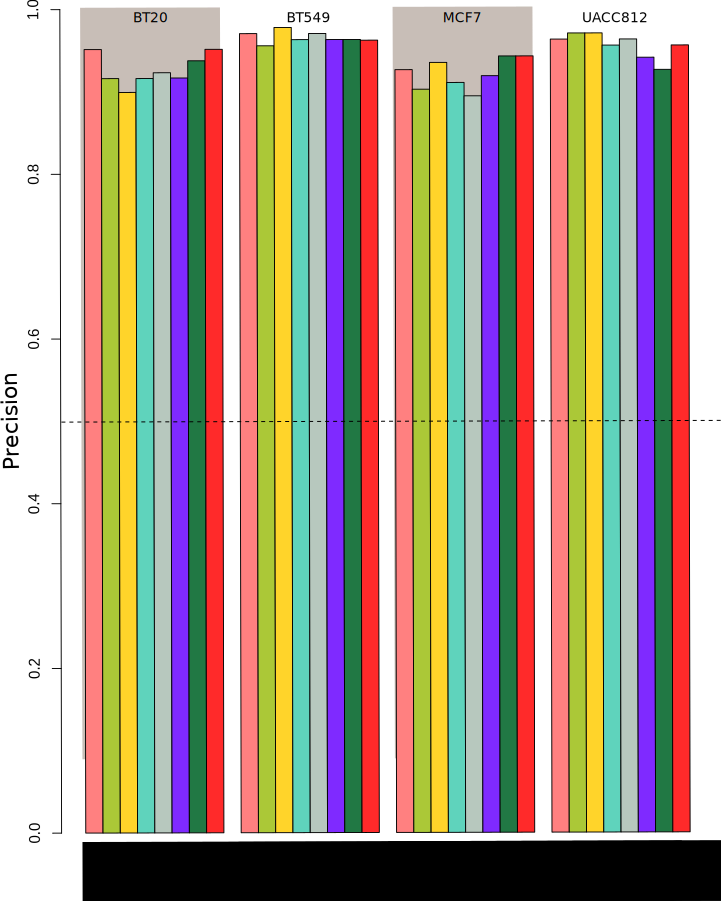
\includegraphics[width=0.4\textwidth]{./Bilder/Precision.pdf}
\caption[Precision]{ }
\label{fig:}
\end{figure}


\section{}


\section{}


    \clearpage{\pagestyle{empty}\cleardoublepage}
    \input{./Kapitel/conclusion}
    \clearpage{\pagestyle{empty}\cleardoublepage}

% -----------------------------------
%\backmatter 
\bibliographystyle{apacite}				% bei natbib in deutsch
\bibliography{./Literatur/quellen}		% Literaturquellen einbinden 
\newpage
\thispagestyle{empty}

\begin{Large}\textbf{Declaration of Originality}\end{Large}\\

\begin{large}

\vspace*{2cm}

\noindent
I hereby declare that this thesis and this work reported herin was composed by and originated entirely from me. Information derived from published and unpublished work of others has been acknowledged in the text and references are given in the list of sources.

\vspace{2cm}

\noindent
Berlin, November 20,2018\\

%\vspace{3cm}

%\hspace*{7cm}%
%\dotfill\\
%\hspace*{8.5cm}%
Nina Valery Kersten

\end{large}
 			% Eidesstattliche Erkl�rung (nicht bei Seminararb.)

\end{document}
